% $Id: groomers-taggers.tex 525 2019-05-13 07:32:20Z smarzani $
%
% This contains an introduction to the jet substructure tools and a
% dictionary of commonly-used methods
%------------------------------------------------------------------------
\chapter{Jet substructure: concepts and tools}\label{tools}

The widest application of jet substructure tools is to disentangle
different kinds of jets. This typically includes separating quark and
gluon-initiated jets or isolating boosted W/Z/H or top jets (our
signal) from the much more abundant QCD background of ``standard''
quark and gluon-initiated jets.
%
In this chapter, we discuss these methods in some detail. We start by considering 
the guiding principles behind the different algorithms and how to assess their performance. 
%
Then, we will review some of
the most commonly-used jet substructure techniques over the past 10
years. 
%
Explicit examples on how these tools behave in Monte-Carlo
simulations and analytic calculations and how they are used in
experimental analyses will be given in the next Chapters.


\section{General guiding principles}\label{sec:tools-generic}

Jet substructure aims to study the internal kinematic 
properties of a high-$p_t$ jet in order to distinguish whether it is more likely to be a signal or  background jet.
%
Although a large variety of methods have been proposed over the last
ten years, they can be grouped into three wide categories, according the physical observation that they mostly rely on.
\begin{description}
\item[{\bf Category I: prong finders.}]
  %
  Tools in this category exploit the fact that when a boosted massive object decays
  into partons, all the partons typically carry a sizeable fraction of
  the initial jet transverse momentum, resulting in multiple hard
  cores in the jet. Conversely, quark and gluon jets are dominated by
  the radiation of soft gluons, and are therefore mainly single-core
  jets.
  %
  Prong finders therefore look for multiple hard cores in a jet, hence
  reducing the contamination from ``standard'' QCD jets.
  %
  This is often used to characterise the boosted jets in terms of their
  ``pronginess'', i.e.\ to their expected number of hard cores:
  QCD jets would be 1-prong objects, W/Z/H jets would be two-pronged,
  boosted top jets would be three-pronged, an elusive new resonance
  with a boosted decay into two Higgs bosons, both decaying to a
  $b\bar b$ pair would be a 4-prong object, ...
  %
\item[{\bf Category II: radiation constraints.}]
  %
  The second main difference between signal and background jets is
  their colour structure. This means that signal and background jets
  will exhibit different soft-gluon radiation patterns. For example, QCD radiation associated with 
  an EW-boson jet, which is colourless, is expected to be less than what we typically find in a QCD jet. 
  Similarly, quark-initiated jets are expected to radiate less
  soft gluons than gluon-initiated jets. Many jet shapes have been
  introduced to quantify the radiation inside a jet and hence separate
  signal jets from background jets.  
  %
\item[{\bf Category III: groomers.}]
  %
  There is a third category of widely-used tools related to the fact
  that one often use large-radius jets for
  substructure studies. As we have already discussed, because of their large area, these jets are particularly sensitive to soft backgrounds, such as the UE and pileup. ``Grooming'' tools have therefore been
  introduced to mitigate the impact of these soft backgrounds on the
  fat jets.
  %
  These tools usually work by removing the soft radiation far from the
  jet axis, where it is the most likely to come from a soft
  contamination rather than from QCD radiation inside the jet.
  %
  In many respects, groomers share similarities with prong finders,
  essentially due to the fact that removing soft contamination and
  keeping the hard prongs are closely related.
  %
  \end{description}
Additionally, we note that we might expect non-trivial interplay between groomers and radiation-constraint observables.
For instance, if we apply observables that exploit radiation constraints on soft
  radiation, to groomed jets, which precisely throws
  away soft radiation, we expect to obtain worse performance. 
  Therefore, we can anticipate that we will have to find a sweet spot between
  keeping the sensitivity to UE and pileup under control, while
  maintaining a large discriminating power.



\section{Assessing performance}\label{sec:performance-intro}

Even though they are based on only a handful of key concepts, a long
list of jet substructure tools have been introduced. Before we dive
into a description of these tools, it is helpful to briefly discuss
how one can compare their relative performance.
%
Note that, here, we are not referring to how the tools can be
validated, which is often done via Monte Carlo studies, direct
measurements in data or analytic studies. Instead, we would like to answer questions like 
 ``There are dozens of tools around, which one should I
use for my problem?'' or ``Which one has the largest performance?''.
%
It is of course impossible to give a definite answer to such
questions, but what we can at least provide is some key ideas of what
we mean by ``performant'' which can be properly tested and quantified.


The case of groomers is the probably the easiest to address, since
groomers have the specific purpose of suppressing the sensitivity to
the UE and pileup.
%
In the case of the UE, we can perform Monte Carlo studies, switching
multiple particle interactions on and off, to check how key distributions --- like the jet
mass distribution in QCD events, W$\to q\bar q$ or hadronic top decay
--- vary.
%
A similar approach applies for pileup, where we can perform Monte
Carlo studies, overlaying minimum bias events with the hard events.
%
In cases where we have access to both a reference event (\eg a hard
collision) and a modified event (\eg the same event overlaid with
pileup), quality measures can then involve average shifts and
dispersions of how jet quantities like the jet mass are affected event
by event.
%
More generally, we can study the position and width of peaks like the
reconstructed W or top mass, and study their stability with respect to the
UE or pileup multiplicity.
%
We refer to Section~4 of Ref.~\cite{Altheimer:2013yza} for an explicit
application of the above procedure.


\begin{figure}
  \centerline{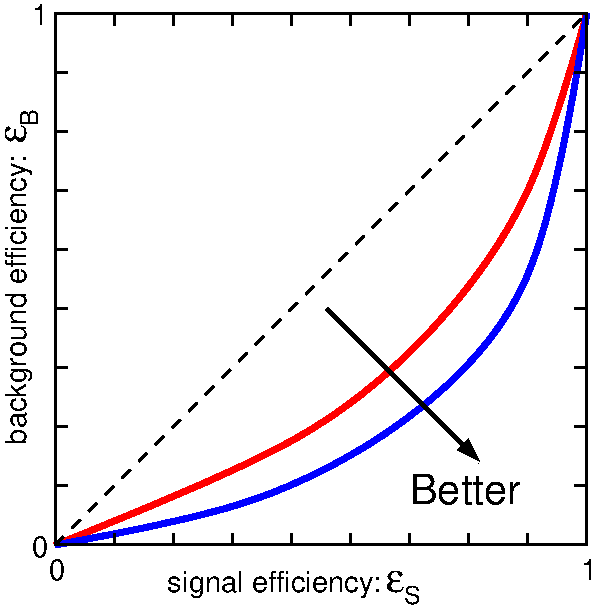
\includegraphics[width=0.45\textwidth]{figures/sketch-roc.pdf}}
  % 
  \caption{A ROC curve represents the background efficiency
    $\epsilon_B$ as a function of the signal efficiency
    $\epsilon_S$. For a given signal efficiency, a lower background
    efficiency is better.}\label{fig:ROC-sketch}
\end{figure}

In the following, we are going to focus on
the case of boosted-object tagging.
%
In this case, there is again a very obvious meaning of what performant
means: the best tool is the one which keeps most of the signal and
rejects most of the background.
%
In practice, for a signal S and a background B, we define the signal
(respectively background) efficiency $\epsilon_S$ ($\epsilon_B$) as
the rate of signal (or background) jets that are accepted by the
tagger. For cases with limited statistics (which is often the case in
searches), the best tool is then the one that maximises the signal
significance, $\epsilon_S/\sqrt{\epsilon_B}$. More generally, for a
given signal efficiency, one would like to have the smallest possible
background rate, \ie for a given amount of signal kept by the tagger,
we want to minimise the rate of background events which wrongly pass
the tagger conditions.
% 
This is usually represented by Receiver Operating Characteristic (ROC)
curves which show $\epsilon_B$ as a function of $\epsilon_S$, such as
represented in Fig.~\ref{fig:ROC-sketch}.
%
This can be used to directly compare the performance of different
substructure tools.

That said, signal significance is not the only criterion one may
desire from a jet substructure tagger.
%
Similarly to the properties of jet definitions discussed in
Chapter~\ref{chap:jets-and-algs}, we may want additional conditions
such as the following:
\vspace*{-0.2cm}
\begin{itemize}
\itemsep0.0cm
\item we would like to work with tools that are infrared and collinear
  safe, \ie which are finite at any order of the perturbation
  theory,\footnote{An interesting class of observables, known as {\it
      Sudakov safe}, fails to fully satisfy this condition but remain
    calculable once a proper all-order calculation is performed (see
    chapter~\ref{sec:curiosities}).}
\item we would like to work with tools that are as little sensitive as possible to model-dependent
  non-perturbative effects such as hadronisation and the Underlying
  Event,
\item we would like to work with tools that are as little sensitive as possible to
  detector effects and pileup.
\end{itemize}
%
In a way, the last two of the above criteria are related to the {\it
  robustness} of our tools, \ie we want to be able to assess how robust our conclusions are
against details of the more poorly-known (compared to
the perturbative part) aspects of high-energy collisions.
%
One should typically expect that a more robust tool would have a
smaller systematic uncertainty associated with theory modelling (\eg
the dependence on which Monte Carlo sample is used), pileup
sensitivity and detector sensitivity/unfolding.\footnote{Small
  systematic uncertainties is really the fundamental assessment of
  robustness. Asking, as we do here, for a small sensitivity to
  non-perturbative and detector effects, is a sufficient condition to
  achieve this, but it is not strictly necessary. One could for
  example imagime a situation where detector effects are large but
  perfectly well understood such that the resulting systematic
  uncertainty remains small.}

Robustness can be quantified in several ways, typically by measuring
how the signal and background efficiencies are affected by a given
effect (see
\eg~\cite{Dasgupta:2016ktv,Salam:2016yht,Bendavid:2018nar}).
%
Some concrete ideas about how to assess robustness were put forward in
Ref.~\cite{Bendavid:2018nar} (Section III.2). Let us say that we want to
test the sensitivity of a tagger with respect to the UE. From a
Monte Carlo simulation, we can compute the signal and background
efficiencies, first without UE, $\epsilon_{S,B}\equiv\epsilon_{S,B}^{(\text{no UE})}$, and then
with UE $\epsilon_{S,B}'\equiv\epsilon_{S,B}^{(\text{UE})}$. We define {\it resilience}, a measure
of robustness, as
\begin{equation}\label{eq:resilience}
  \zeta = \left(
      \frac{\Delta\epsilon_{S}^2}{\left\langle\epsilon\right\rangle_{S}^2}
    + \frac{\Delta\epsilon_{B}^2}{\left\langle\epsilon\right\rangle_{B}^2}
  \right)^{-1/2}
\end{equation}
where
\begin{equation}
  \Delta \epsilon_{S,B}  =\epsilon_{S,B}-\epsilon_{S,B}'
  \qquad\text{ and }\qquad
\left\langle\epsilon\right\rangle_{S,B} 
     =\frac{1}{2}\left(\epsilon_{S,B}+\epsilon_{S,B}'\right).
\end{equation}
With this definition, a large resilience means that the signal and
background efficiencies have not changed much when switching the UE on
and hence that the tool is robust.
%
Resilience can be defined for hadronisation, \ie when switching on
hadronisation and going from parton level to hadron level, for the UE,
as discussed above, for pileup sensitivity, \ie when overlaying the
event with pileup and applying a pileup mitigation technique, and for
detector sensitivity, \ie when running events through a detector
simulation.

To conclude, it is important to realise that the performance of a jet
substructure tagger is characterised by several aspects. Performance,
typically quantified by ROC curves of signal significance is certainly
the most regarded feature of a tagger. However, other requirements
like the robustness against non-perturbative effects, pileup and
detector effects are desirable as well. These can be quantified \eg
via resilience.

\section{Prong-finders and groomers}\label{sec:tools-prong-finders-groomers}


\paragraph{Mass-drop tagger.} The Mass-Drop
tagger was originally proposed~\cite{Butterworth:2008iy} as a tool to
isolate boosted Higgs bosons, decaying to $b\bar b$ pairs, from the
QCD background. 
In this procedure, one first reclusters the jet constituents of the fat
jet with the Cambridge/Aachen algorithm. One then iteratively undoes
the last step of the clustering $p_{i+j}\to p_i+p_j$ and check the
following criteria: (i) there is a ``mass drop'' \ie
${\rm max}(m_i,m_j)<\mu_{\rm cut}m_{i+j}$, (ii) the splitting is
sufficiently symmetric \ie
${\rm min}(p_{t,i}^2,p_{t,j}^2)\Delta R_{ij}^2>y_{\rm cut} m_{i+j}^2$.
When both criteria are met, we keep ``$i+j$'' as the result of the
mass-drop tagger, otherwise the least massive of $i$ and $j$ is
discarded and the procedure is repeated iteratively using the most
massive of $i$ and $j$.\footnote{If the procedure fails to find two
  subjets satisfying the conditions, \ie end up recursing until it
  reaches a single constituent which can not be further de-clustered,
  it is considered as having failed and returns an empty jet.}
%
The mass-drop tagger has two parameters: $\mu_{\rm cut}$, the
mass-drop parameter itself, and $y_{\rm cut}$, the symmetry cut.
%
The two conditions imposed by the mass-drop tagger exploit the
fundamental properties introduced above for tagging two-pronged
boosted objects: the symmetry cut requires that one indeed finds two
hard prongs and the mass-drop condition imposes that one goes from a
massive boson jet to two jets originated from massless QCD partons.
% 
Although it was originally introduced as a tagger, the mass-drop
tagger also acts as a groomer since, following the declustering
procedure, it would iteratively remove soft radiation at the
outskirts of the jet, hence reducing the pileup/UE contamination.

\paragraph{modified Mass-Drop Tagger (mMDT).} When trying to understand the
analytic behaviour of the mass-drop tagger on QCD jets, it was
realised that following the most massive branch in the iterative
de-clustering procedure leads to pathological situations. It was
therefore suggested~\cite{Dasgupta:2013ihk} to adapt the procedure so
that it instead follows the hardest branch (in terms of $p_t$).
%
This modification makes the analytical calculation much easier and
more robust without affecting the performance of the method (even
improving it slightly).
%
The same study also added two more minor modifications. First, it was
realised that the symmetry condition could be replaced by
${\rm min}(p_{t,i},p_{t,j})>z_{\rm cut}(p_{t,i}+p_{t,j})$ which has
the same leading analytic behaviour as the $y_{\text{cut}}$ condition
and a slightly reduced sensitivity to non-perturbative
corrections. Second, the mass-drop condition would only enter as a
subleading correction in the strong coupling constant $\alpha_s$,
compared to the symmetry condition. It can therefore usually be
ignored.


\paragraph{\SD.} \SD~\cite{Larkoski:2014wba} can be seen a
generalisation of mMDT. It also proceeds by
iteratively declustering a jet reclustered with the Cambridge/Aachen
algorithm but replaces the symmetry condition for the
declustering of $p_{i+j}$ into $p_i$ and $p_j$, with
\begin{equation}\label{eq:soft-drop-condition}
  \frac{{\rm min}(p_{t,i},p_{t,j})}{p_{t,i}+p_{t,j}} 
    > \zcut \left(\frac{\Delta R_{ij}}{R}\right)^\beta,
\end{equation}
where $R$ is the jet radius.
%
\SD has two parameters. The $\zcut$ parameter plays the same role as
in the (m)MDT of keeping the hard structure and excluding soft
emissions, starting from large angles.
%
The $\beta$ parameter gives \SD some extra freedom in controlling how
aggressive the groomer is.
%
In the limit $\beta\to 0$, \SD reduces to the mMDT. Increasing $\beta$
leads to a less aggressive grooming procedure, with $\beta \to \infty$
corresponding to no grooming at all. Conversely, choosing a negative
value for $\beta$ would lead a more aggressive two-prong tagger than
mMDT.\footnote{The \SD procedure returns by default a single particle
  if it fails to find two subjets satisfying the \SD condition. This
  ``grooming mode'' is different from the default ``tagging mode'' of
  the mMDT which would fail, \ie return an empty jet, if no
  substructure are found.}
%
For practical applications, mMDT and \SD with negative $\beta$
(typically $\beta=-1$) would, alone, be perfectly adequate and
efficient taggers (see e.g. Section 7 of Ref.~\cite{Larkoski:2014wba})

\paragraph{Recursive \SD.} \SD typically finds two prongs in a jet. If we want to find more than two prongs, we can apply \SD
recursively. Recursive \SD~\cite{Dreyer:2018tjj} does this by
iteratively undoing the clustering with the largest $\Delta R$ in the
Cambridge/Aachen tree. Both branches are kept if the \SD
condition~(\ref{eq:soft-drop-condition}) is met and the softer branch
is dropped otherwise. The procedure stops when $N+1$ prongs have been
found, with $N$ an adjustable parameter that can be taken to infinity.

\paragraph{Filtering.} Filtering was first introduced in
Ref.~\cite{Butterworth:2008iy} as a grooming strategy to clean the jet
from UE after the mMDT has been applied. For a given jet, it
re-clusters its constituents with the Cambridge/Aachen algorithm with
a small radius $R_{\rm filt}$ and only keeps the $n_{\rm filt}$ larger
$p_t$ subjets. The subjets that have been kept constitute filtered jet.
%
This has two adjustable parameters: $R_{\rm filt}$ and $n_{\rm filt}$.
%
It is typically used to reduce soft contamination in situations where
we have a prior knowledge of the number of hard prongs in a
jet. For a jet with $n_{\rm prong}$ hard prongs --- $n_{\rm prong}=2$
for a $W/Z/H$ bosons and $n_{\rm prong}=3$ for a top --- we would
typically use $n_{\rm filt}=n_{\rm prong}+1$ which would also keep the
(perturbative) radiation of an extra gluon.

\paragraph{Trimming.} Trimming~\cite{Krohn:2009th} shares some
similarities with filtering. It also starts with re-clustering the jet
with a smaller radius, $R_{\rm trim}$, using either the $k_t$ or the
Cambridge/Aachen algorithm. It then keeps all the subjets with a
transverse momentum larger than a fraction $f_{\rm trim}$ of the
initial jet transverse momentum.
%
On top of the choice of algorithm, this also has two parameters:
$R_{\rm trim}$ and $f_{\rm trim}$.
%
It is often used both as a generic groomer and as a prong finder in boosted-jet
studies.


\paragraph{Pruning.} Pruning~\cite{Ellis:2009su} is similar in spirit
to trimming but it adopts a bottom-up approach (with trimming seen as
a top-down approach). Given a jet, pruning reclusters its constituents
using a user-specified jet definition (based on pairwise
recombinations) and imposes a constraint at each step of the
clustering: objects $i$ and $j$ are recombined if they satisfy at
least one of these two criteria: (i) the geometric distance
$\Delta R_{ij}$ is
smaller than
$R_{\rm prune}=2 f_{\rm prune} m_{\rm jet}/p_{t,\rm jet}$, with
$p_{t,\rm jet}$ and $m_{\rm jet}$ the original jet transverse momentum
and jet mass, (ii) the splitting between $i$ and $j$ is sufficiently
symmetric, \ie
${\rm min}(p_{t,i},p_{t,j})\ge z_{\rm prune}p_{t,(i+j)}$. If neither criteria are met, only the hardest of $i$ and $j$ (in terms of
their $p_t$) is kept for the rest of the clustering and the other is
rejected.
%
On top of the jet definition used for the re-clustering, which is
usually taken to be either $k_t$ or Cambridge/Aachen with a radius
much larger than the one of original jet, this has two parameters:
$f_{\rm prune}$ and $z_{\rm prune}$. 
%
$z_{\rm prune}$ plays the same role as $f_{\rm trim}$ for trimming and
$f_{\rm prune}$ plays a role similar to $R_{\rm trim}$. Note that, in
the case of pruning, $R_{\rm prune}$ is defined dynamically based on the
jet kinematics, while $R_{\rm trim}$ is kept fixed. This can have
important consequences both analytically and phenomenologically.
%
Pruning can be considered as a general-purpose groomer and tagger
and is often used in situations similar to trimming, although it tends
to be slightly more sensitive to pileup contamination.

\paragraph{I and Y-Pruning.} When pruning a jet, there might be
situations where a soft emission at large angle dominates the mass of
the jet, thus setting the pruning radius, but gets pruned away because it does not satisfy the pruning
conditions. The mass of the pruned jet is then determined by radiation
at smaller angle, typically within the pruning radius. This situation
where the jet mass and the pruning radius are determined by different
emissions in the jet would result in a jet with a single prong, and it usually referred to 
called ``I-pruning"~\cite{Dasgupta:2013ihk}. For I-pruning, the pruning radius does not have the
relation to the hard substructure of the jet it is intended to.

More precisely, I-Pruning is defined as the
subclass of pruned jets for which, during the sequential clustering,
there was never a recombination with $\Delta R_{ij}>R_{\rm prune}$ and
${\rm min}(p_{t,i},p_{t,j})> z_{\rm prune}p_{t,(i+j)}$.
%
The other situation, \ie a pruned jet for which there was at least one
recombination for which $\Delta R_{ij}>R_{\rm prune}$ and
${\rm min}(p_{t,i},p_{t,j})> z_{\rm prune}p_{t,(i+j)}$, corresponds to
a genuine two-prong structure and is called Y-Pruning.

This distinction between I- and Y-Pruning is mostly irrelevant for
boosted jet tagging. However, it has been shown to have an impact on
the analytical behaviour of Pruning, with Y-Pruning being under better
control and than I-Pruning, the latter adding an extra layer of
complexity to the calculation. If one's goal is to reach some level of
analytic control over groomed jets, Y-Pruning appears as a more
natural choice than Pruning which also includes the contribution from
I-Pruning.

\paragraph{Y-Splitter.} Y-Splitter is one of the very few tools
proposed for boosted W-boson tagging at the
LHC~\cite{Butterworth:2002tt}.
%
The idea is to recluster the constituents of the jet with the $k_t$
algorithm and to undo the last step of the clustering. This gives two
subjets $j_1$ and $j_2$. One then defines
\begin{equation}
y_{12} = \frac{k_{t,12}^2}{m_{12}^2} = \frac{{\rm
    min}(p_{t1}^2,p_{t2}^2)\Delta R_{12}^2}{m_{12}^2},
\end{equation}
similar to what has been used later in the MassDrop Tagger. One then
imposes the cut $y>y_\text{cut}$ to require to hard prongs in the
jet.\footnote{A cut on $y$ is roughly equivalent to a cut on the $p_t$
  fraction $z$. For example, for a jet made of two collimated partons
  carrying a momentum fraction $z$ and $1-z$ of the jet, one has
  $y=\tfrac{z}{1-z}$.}
Note that similar quantities have been introduced as event shapes in
$e^+e^-$ collisions.

\paragraph{Johns Hopkins top tagger.} As its name suggests, this is a
tagger meant to separate fat jets originating from the decay of
boosted top quarks from the background made of light-quark jets.
%
It was one of the first substructure techniques introduced in the
context of LHC physics.
%
The tagger aims at finding three hard prongs in the jet, corresponding
to the $q\bar q b$ hard quarks produced by the hadronic decay of the
top, adding constraints that two of the three prongs are compatible
with a hadronically-decaying W boson.
%
In practice, it proceeds as follows~\cite{Kaplan:2008ie}:
%
\begin{enumerate}
\item If the initial jet has not been obtained by the Cambridge/Aachen
  algorithm, re-cluster the jet constituents using this algorithm,
  % 
\item {\em Primary decomposition}: as for the mMDT, we iteratively
  undo the last step of the Cambridge/Aachen clustering. The softer of the two
  subjets is discarded if its transverse momentum divided by the {\em
    initial} jet $p_t$ is smaller than a parameter $\delta_p$. The
  de-clustering procedure then continues with the harder subjet.
  %
  This is repeated until one of our things happens: (i) both subjets are
  above $\delta_p$, (ii) both subjets are below $\delta_p$, (iii) the
  two subjets satisfy $|\Delta y|+|\Delta \phi|<\delta_r$, with
  $\delta_r$ another parameter of the tagger, or (iv) the subjet can
  no longer be declustered. In case (i) the two hard subjets are kept
  and further examined, in the other three cases, the jet is not
  tagged as a top candidate.
  %
\item {\em Secondary decomposition}: with the two prongs found by the
  primary decomposition, repeat the declustering procedure as for the
  primary decomposition, still defining the $\delta_p$ condition with respect to
  the original jet $p_t$.
  % 
  This can result in either both prongs from the primary decomposition
  being declustered into two sub-prongs, only one prong being
  declustered, or none.
  % 
  When no further substructure is found in a primary prong, the
  primary prong is kept intact in the final list of prongs. When two
  sub-prongs are found both are kept in the final list of prongs.
  % 
  Ultimately, this leads to two, three or four prongs emerging from
  the original jet. Only jets with three or four sub-prongs are then
  considered as top candidates, while the case with only two prongs is
  rejected.
  %
\item {\em Kinematic cuts}: with the three or four prongs found from
  the secondary decomposition, impose additional kinematic
  conditions. First, the sum of the four-momenta of all the hard
  prongs should be close to the top mass. Then, there exists two
  prongs which invariant mass is close to the W mass. Finally we
  impose that the W helicity angle be consistent with a top
  decay.
  %
  The W helicity angle, $\theta_h$, is defined as the angle between
  the top direction and one of the W decay products, in the rest
  frame of the W. We impose $\cos(\theta_h)<0.7$.\footnote{Top decays are almost isotropic and the helicity angle had
    an almost flat distribution, while for QCD jets, it diverges like
    $1/(1-\cos(\theta_h))$.}
\end{enumerate}
%
The original paper suggested that the parameters should be adjusted according to the
event's scalar $E_T$:
\begin{align}
  1~\text{TeV}<E_T<1.6~\text{TeV}:\;   & R=0.8, && \delta_p=0.10, && \delta_r=0.19, \\ 
  1.6~\text{TeV}<E_T<2.6~\text{TeV}:\; & R=0.6, && \delta_p=0.05, && \delta_r=0.19, \\
  2.6~\text{TeV}<E_T:\;                & R=0.4, && \delta_p=0.05, && \delta_r=0.19. 
\end{align}
The kinematic cuts are then adjusted based on the jet $p_t$:
\begin{align}
  p_t<1~\text{TeV: } & 145<m_\text{top}<205~\text{GeV}, && 65<m_{W}<95~\text{GeV}, \\ 
  p_t>1~\text{TeV: } & 145<m_\text{top}<p_t/20+155~\text{GeV}, && 65<m_{W}<70+p_t/40~\text{GeV},
\end{align}
where $m_\text{top}$ and $m_W$ are the reconstructed top and W mass respectively.

The prong decomposition of the Johns Hopkins top tagger shared
obvious similarities with the (modified) MassDrop Tagger introduced to
tag Higgs bosons, in the sense that it follows the hardest branch on a
Cambridge/Aachen clustering tree and imposes a hardness condition on
the subjets. Since we now want to require three hard prongs in the
jet, the de-clustering procedure is repeated twice. The main
noticeable differences between the (modified) MassDrop Tagger and the
Johns Hopkins top tagger is that the latter imposes a $\delta_p$
condition computed with respect to to the original jet $p_t$ while the mMDT
imposes its $\zcut$ condition computed as a fraction of the subjets
parent's $p_t$.
%
Note also the use of the Manhattan distance in the $\delta_r$
condition.

In practice, for a top efficiency between 20 and 40\%, the Johns
Hopkins top tagger achieves reductions of the background by a factor
$\sim 100$ (remember these numbers should be squared for the
efficiency to tag a $t\bar t$ pair).

\paragraph{CMS top tagger.}  The CMS top tagger is essentially an
adaptation of the Johns Hopkins top tagger proposed by the CMS
collaboration~\cite{CMS:2009lxa,CMS:2014fya}. Declustering proceeds analogously to the Johns Hopkins top tagger --- except for the
two-prongs distance condition which uses a $p_t$-dependent cut on the
standard $\Delta R_{ij}$ subjet distance ---, but the kinematic
conditions are different. The detailed procedure works as follows:
%
\begin{enumerate}
\item If needed, the initial jet is re-clustered using the Cambridge/Aachen
  algorithm.
%
\item {\em Primary decomposition}: the last step of the clustering is
  undone, giving two prongs. These two prongs are examined for the
  condition
  \begin{equation}\label{eq:cms-top-cdt}
    p_t^{\mathrm{prong}} > \delta_p \, p_t^{\text{jet}},
  \end{equation}
  where $p_t^{\text{jet}}$ refers to the hard jet transverse
  momentum. $\delta_p$ is a parameter which is usually taken as
  $0.05$.
  % 
  If both prongs pass the cut then the ``primary'' decomposition
  succeeds.
  %
  If both prongs fail the cut then the jet is rejected \ie is not
  tagged as a top jet.
  %
  If a single prong passes the cut the primary decomposition recurses
  into the passed prong, until the decomposition succeeds or the whole
  jet is rejected.
  %
  Note that during the recurrence, $p_t^{\text{jet}}$ (used in
  (\ref{eq:cms-top-cdt})) is kept as the transverse momentum of the
  original jet.
  % 
\item {\em Secondary decomposition}: with the two prongs found by the
  primary decomposition, repeat the declustering procedure as for
  the primary decomposition, still defining the $\delta_p$
  condition~\eqref{eq:cms-top-cdt} with respect to the original jet $p_t$.
  % 
  This can result in either both prongs from the primary decomposition
  being declustered into two sub-prongs, only one prong being
  declustered, or none.
  % 
  When no further substructure is found in a primary prong, the
  primary prong is kept intact in the final list of prongs. When two
  sub-prongs are found both are kept in the final list of prongs.
  % 
  Ultimately, this leads to two, three or four prongs emerging from
  the original jet. Only jets with three or four sub-prongs are then
  considered as top candidates.
  %
\item {\em Kinematic constraints}: taking the three highest $p_t$
  subjets (\ie prongs) obtained by the declustering, find the minimum
  pairwise mass and require this to be related to the W mass, $m_W$,
  by imposing the condition
  $\mathrm{min} \left(m_{12},m_{13},m_{23} \right) > m_{\mathrm{min}}
  $ with $m_{\mathrm{min}} \lesssim m_W$.
  % 
  For practical applications, $m_{\text{min}}$ is usually taken as
  $50$~GeV.
  % 
\item Note that in the second version of the
  tagger~\cite{CMS:2014fya}, the decomposition procedure also imposes
  an angular cut: when examining the decomposition of a subjet $S$
  into two prongs $i$ and $j$, the CMS tagger also requires
  $\Delta R_{ij} > 0.4 - A p_t^S$ where
  $\Delta R_{ij} = \sqrt{\Delta y_{ij}^2+ \Delta \phi_{ij}^2}$ and
  $p_t^S$ refers to the transverse momentum of the
  subjet.
  % 
  The default value for $A$ is $0.0004 \, \mathrm{GeV^{-1}}$.
  %
  We note that without a $\Delta R$ condition in the decomposition of
  a cluster, the CMSTopTagger is collinear unsafe
  (see~\cite{Dasgupta:2018emf} for a discussion of this and proposed
  alternatives).
\end{enumerate}




\section{Radiation constraints}\label{sec:tools-radiation-constraints}

The standard approach to constraining radiation inside a jet is to
impose a cut on a {\em jet shape} which, similarly to event shapes in
electron-positron collisions, is sensitive to the distribution of the particles in the jet
(or in the event for the $e^+e^-$ case).
%
Over the past ten years, several jet shapes have been introduced. In what follows,  we
review the most common ones.

\subsection{Angularities and generalised angularities}\label{sec:def-angularities}

The simplest family of jet shapes is probably the {\em generalised
  angularities}~\cite{Larkoski:2014pca} defined as
\begin{equation}\label{eq:generalised-angularities}
  \lambda_\beta^\kappa = \sum_{i\in\jet} z_i^\kappa
    \left(\frac{\Delta R_{i,\jet}}{\\R}\right)^\beta,
\end{equation}
where $z_i$ is the jet transverse momentum fraction carried by the
constituent $i$ and $\Delta R_{i,\jet}$ its distance to the jet axis:
\begin{equation}
  z_i = \frac{p_{t,i}}{\sum_{j\in\jet}p_{t,j}}
  \qquad\text{ and }\quad
  \Delta R_{i,\jet}^2 = (y_i- y_{\jet})^2 + (\phi_i- \phi_{\jet})^2.
\end{equation}
Note that generalised angularities (and more in general, the other jet shapes
presented later) can also be used for jets in $e^+e^-$
collisions if we define $z_i=E_i/E_\jet$ and replace
$\Delta R_{i,\jet}$ either by $\theta_{i,\jet}$, the angle to the jet
axis, or by
$2\sin(\theta_{i,\jet}/2)=\sqrt{2(1-\cos \theta_{i,\jet})}$.

Generalised angularities are collinear unsafe, except for the special
case $\kappa=1$ which corresponds to the IRC safe 
{\em angularities}~\cite{Berger:2003iw,Almeida:2008yp}:
\begin{equation}\label{eq:angularities}
\lambda_\beta \equiv \lambda_\beta^{(\kappa=1)}.
\end{equation}
The specific case $\beta=1$ is sometimes referred to as {\em width} or
{\em girth} or {\em broadening}, while $\beta=2$ is closely related to
the jet mass.\footnote{It reduces to $\rho=m^2/(p_tR)^2$ in the limit
  of massless particles and small jet radius $R$.}


Obviously, the more radiation there is in a jet, the larger generalised
angularities are. 
%
Angularities and generalised angularities can therefore be seen as a
measure of QCD radiation around the jet axis, \ie as the radiation
in a one-pronged jet. They are often used as a quark-gluon
discriminator, where gluon-initiated jets would, on average, have
larger angularity values that quark-initiated
jets~\cite{Gallicchio:2011xq,Gallicchio:2012ez,Badger:2016bpw}.


For completeness, we note that the ``jet'' axis used to compute
angularities can differ from the axis obtained via the initial
jet clustering (usually the anti-$k_t$ algorithm with jet radius $R$
and $E$-scheme recombination). A typical example is the case of the jet
width where using an axis defined with the $E$-scheme recombination
introduces a sensitivity to recoil and complicates the analytic
calculations of width. The workaround is to use a recoil-free axis,
like the WTA recombination scheme. More generally, it is advisable to use the
WTA axis for angular exponents $\beta\le 1$. This is also valid for
the other shapes defined below and we will adopt this choice when presenting
analytic calculations.

There are at least two other examples of generalised angularities
that, despite being IRC unsafe, are widely used in applications. The
case $\beta=\kappa=0$ corresponds to the {\em jet multiplicity}, and
$\beta=0$, $\kappa=2$, which is related to
$p_t^D$~\cite{Pandolfi:1480598,Chatrchyan:2012sn}.
%
Finally, generalised angularities can be defined as track-based
observables by limiting the sum in
Eq.~(\ref{eq:generalised-angularities}) to the charged tracks (\ie
charged constituents) in the jet. Tracked-based angularities are
advantageous in the context of pileup mitigation, because compared to
neutral energy deposits in calorimeters, it is easier to separate
tracks that originate from pileup vertices from tracks from the
hard-interaction. The price we pay is that tracked-based observables
are not IRC safe and theoretical predictions involve non-perturbative
fragmentation
functions~\cite{Chang:2013rca,Chang:2013iba,Elder:2018mcr}.

\subsection{$N$-subjettiness}\label{sec:def-Nsubjettiness}
As the name suggests, $N$-subjettiness~\cite{Thaler:2010tr} is a jet shape that aims to discriminate jets according to the number $N$ of subjets they are made of. 
It takes inspiration from the event-shape $N$-jettiness~\cite{Stewart:2010tn}.
In order to achieve this, a set of axes $a_1,\dots,a_N$ is introduced (see below for a more precise
definition) and the following jet shape is introduced~\footnote{Eq.~\eqref{eq:Nsubjettiness} corresponds to the {\em
    un-normalised} definition of $N$-subjettiness. Alternatively, one
  can normalise $\tau_N$ by the jet scalar $p_t$,
  $\tilde p_t=\sum_{i\in\jet}p_{ti}$, or, more simply, the jet $p_t$.}
\begin{equation}\label{eq:Nsubjettiness}
  \tau_N^{(\beta)} = \sum_{i\in\jet} p_{ti}\,
  {\text{min}}(\Delta R_{ia_1}^\beta,\dots,\Delta R_{ia_N}^\beta),
\end{equation}
where $\beta$ is a free parameter.\footnote{Although it is strongly
advised to specify the value of $\beta$ one uses, $\beta=1$ is
often implicitly assumed in the literature.}
%
The axes $a_i$  can be defined in several ways, the most common
choices being the following:
\begin{itemize}
\item {\bf $k_t$ axes}: the jet is re-clustered with the $k_t$
  algorithm and the $a_i$ are taken as the  $N$ exclusive jets.
  %
\item {\bf WTA $k_t$ axes}: the jet is re-clustered with the $k_t$
  algorithm, using the winner-take-all recombination scheme. The $a_i$
  are taken as the $N$ exclusive jets. As for angularities, the
  use of the WTA axes guarantees a recoil-free observable.
  %
\item {\bf generalised-$k_t$ axes}: this is defined as above but now
  one uses the exclusive jets obtained with the generalised $k_t$
  algorithm.
  %
  It is helpful to set the $p$ parameter of the generalised $k_t$
  algorithm to $1/\beta$, so as to match the distance measure used for
  the clustering with the one used to compute $\tau_N$.
  %
  For $\beta<1$ one would again use the WTA generalised-$k_t$ axes.
  %
\item {\bf minimal axes}: chose the axes $a_i$ which minimise the
  value of $\tau_N$. The minimum is found by iterating the
  minimisation procedure described in Ref.~\cite{Thaler:2011gf}
  starting with a set of seeds. It is often possible to find a less
  computer-expensive definition (amongst the other choices listed
  here) which would be as suitable to the minimal axes, both for
  phenomenological applications and for analytic calculations.
  %
\item {\bf one-pass minimisation axes}: instead of running a full
  minimisation procedure as for the minimal axes, one can instead
  start from any other choice of axes listed above and run the
  minimisation procedure described in Ref.~\cite{Thaler:2011gf}.
\end{itemize}

As for the angularities discussed in the previous section, $\tau_N$ is
a measure of the radiation around the $N$ axes $a_1,\dots,a_N$. For a
jet with $N$ prongs, one expects $\tau_1,\dots,\tau_{N-1}$ to be
large and $\tau_{\ge N}$ to be small. The value of $\tau_N$ will also
be larger when the prongs are gluons. For these reasons, the
$N$-subjettiness ratio
\begin{equation}\label{eq:tau_ratios}
  \tau_{N,N-1}^{(\beta)} = \frac{\tau_N^{(\beta)}}{\tau_{N-1}^{(\beta)}}
\end{equation}
is a good discriminating variable for $N$-prong signal jets against
the QCD background.
%
More precisely, one would impose a cut
$\tau_{21}^{(\beta)}<\tau_{\text{cut}}$ to discriminate W/Z/H jets
against QCD jets and $\tau_{32}^{(\beta)}<\tau_{\text{cut}}$ to
discriminate top jets against QCD jets
%
Although the most common use of $N$-subjettiness in the literature
takes $\beta=1$, there are also some motivations to use $\beta=2$, see
e.g.~\cite{Larkoski:2013eya,Salam:2016yht}.


\subsection{Energy-Correlation Functions}\label{sec:def-ecfs}

Energy-correlation functions (ECFs) achieve essentially the same objective
than $N$-subjettiness without requiring the selection of $N$
reference axes.
%
In their original formulation~\cite{Larkoski:2013eya}, they are defined as
\begin{align}
e_2^{(\beta)} &= \sum_{i<j\in\jet} z_i z_j \,\Delta R_{ij}^\beta,\label{eq:ecf-e2}\\
e_3^{(\beta)} &= \sum_{i<j<k\in\jet} z_i z_j z_k \,\Delta
                R_{ij}^\beta \Delta R_{jk}^\beta \Delta R_{ik}^\beta,\label{eq:ecf-e3}\\
 &\vdots\nonumber\\
e_N^{(\beta)} &= \sum_{i_1<...<i_N\in\jet} \bigg(\prod_{j=1}^Nz_{i_j}\bigg)
                \bigg(\prod_{k<\ell=1}^N\Delta R_{i_ki_\ell}^\beta\bigg),\label{eq:ecf-eN}
\end{align}
with $z_i=p_{t,i}/\sum_j p_{t,j}$.
%
Compared to $N$-subjettiness, energy-correlation functions have the
advantage of not requiring a potentially delicate choice of reference
axes. Furthermore, from an analytic viewpoint, they are insensitive to
recoil for all values of the angular exponent $\beta$, allowing for an easier analytic
treatment (although, as we have mentioned earlier, this issue can be alleviated in the
$N$-subjettiness case by using WTA axes).

Generalised versions of the
angularities have been introduced~\cite{Moult:2016cvt}. They still involve $p_t$ weighted
sums over pairs, triplets,... of particles but are built from other
angular combinations:
\begin{align}
  {}_1e_2^{(\beta)} &\equiv e_2,\\
  {}_3e_3^{(\beta)} &\equiv e_3,\\
  {}_2e_3^{(\beta)} &= \sum_{i<j<k\in\jet} z_i z_j z_k
            \:\text{min}\big(
            \Delta R_{ij}^\beta \Delta R_{ik}^\beta
            \Delta R_{ij}^\beta \Delta R_{jk}^\beta
            \Delta R_{ik}^\beta \Delta R_{jk}^\beta\big), \\
  {}_1e_3^{(\beta)} &= \sum_{i<j<k\in\jet} z_i z_j z_k
            \:\text{min}\big(
            \Delta R_{ij}^\beta,\Delta R_{ik}^\beta,\Delta R_{jk}^\beta\big), \\
 &\vdots\nonumber\\
  {}_ke_N^{(\beta)} &= \sum_{i_1<...<i_N\in\jet} \bigg(\prod_{j=1}^Nz_{i_j}\bigg)
                \bigg(\prod_{\ell=1}^k
            \underset{u<v\in\{i_1,...,i_N\}}{\overset{\ell}{\text{min}}} \Delta R_{uv}^\beta\bigg),
\end{align}
where $\overset{\ell}{\text{min}}$ denotes the $\ell$-th smallest number.

Similarly to $N$-subjettiness, in order to discriminate boosted massive particles from background QCD jets,
we again introduce ratios of (generalised-)ECFs. Over the past few years,
several combinations have been proposed. Examples of ratios of ECFs that are used as two-prong taggers include
\begin{align}
  C_2^{(\beta)} &= \frac{{}_3e_3^{(\beta)}}{\big({}_1e_2^{(\beta)}\big)^2}
                  \equiv
                  \frac{e_3^{(\beta)}}{\big(e_2^{(\beta)}\big)^2},
                  &
  D_2^{(\beta)} &= \frac{e_3^{(\beta)}}{\big(e_2^{(\beta)}\big)^3},\\
  N_2^{(\beta)} &=  \frac{{}_2e_3^{(\beta)}}{\big(e_2^{(\beta)}\big)^2},
                  &
  M_2^{(\beta)} &= \frac{{}_1e_3^{(\beta)}}{e_2^{(\beta)}},\nonumber
\end{align}
while for three-prong tagging, one introduces~\cite{Larkoski:2013eya,Larkoski:2014zma,Moult:2016cvt}
\begin{align}
  C_3^{(\beta)} &= \frac{e_4^{(\beta)}e_2^{(\beta)}}{\big(e_3^{(\beta)}\big)^2},\qquad\qquad\qquad
  N_3 = \frac{{}_2e_4^{(\beta)}}{\big({}_1e_3^{(\beta)}\big)^2},\qquad\qquad\qquad
  M_3 = \frac{{}_1e_4^{(\beta)}}{{}_1e_3^{(\beta)}},\\
  D_3^{(\alpha,\beta,\gamma)}
    &=\frac{e_4^{(\gamma)}\big(e_2^{(\alpha)}\big)^{\frac{3\gamma}{\alpha}}}
           {\big(e_3^{(\beta)}\big)^{\frac{3\gamma}{\beta}}}
     +\kappa_1\Big(\frac{p_t^2}{m^2}\Big)^{\frac{\alpha\gamma}{\beta}-\frac{\alpha}{2}}
      \frac{e_4^{(\gamma)}\big(e_2^{(\alpha)}\big)^{\frac{2\gamma}{\beta}-1}}
           {\big(e_3^{(\beta)}\big)^{\frac{2\gamma}{\beta}}}
     +\kappa_2\Big(\frac{p_t^2}{m^2}\Big)^{\frac{5\gamma}{2}-2\beta}
      \frac{e_4^{(\gamma)}\big(e_2^{(\alpha)}\big)^{\frac{2\beta}{\alpha}-\frac{\gamma}{\alpha}}}
           {\big(e_3^{(\beta)}\big)^2},\nonumber
\end{align}
where $\kappa_1$ and $\kappa_2$ are ${\cal{O}}(1)$ constants.

In this series, the $D$ family has typically a larger
discriminating power, at the expense of being more sensitive to
model-dependent soft contamination in the jet like the UE
or pileup.
%
Instead, the $N$ family is closer to $N$-subjettiness, and the $M$
family is less discriminating but more resilient against soft
contamination in the jet.

Finally, we note that Energy Correlation functions have recently been
extended into Energy Flow polynomials~\cite{Komiske:2017aww} which
provide a linear basis for all infrared-and-collinear-safe jet
substructure observables. These can then be used to design Energy Flow
Networks~\cite{Komiske:2018cqr} which are QCD-motivated
machine-learning substructure tools.

\subsection{Additional shapes}\label{sec:def-other-shapes}

Over the past decade, several other jet shapes have been introduced in
the literature and studied by the LHC experiments. Since they tend to
be less used than the ones introduced above, we just briefly list the
most common ones below, without entering into a more detailed
discussion.

\paragraph{Iterated \SD.} This is related to Recursive \SD
introduced earlier. The idea is still to apply \SD multiple
times except that this time we will only follow the hardest branch in
the recursion procedure~\cite{Frye:2017yrw}. This gives a list of
branchings which pass the \SD condition,
$(z_1,\theta_1), \dots, (z_n,\theta_n)$, from which we can build
observables. The most interesting observable is probably the {\em
  Iterated \SD multiplicity}, which is simply the number of branchings
which have passed the \SD condition and which is an efficient
quark-gluon discriminator as we will show in
chapter~\ref{sec:calc-shapes-qg}.
%
Alternatively, we can build Iterated \SD angularities from the set of
$(z_i,\theta_i)$.
%
We note that for the Iterated SoftDrop multiplicity to be infrared
and collinear safe, we need either to take a negative value of the \SD
parameter $\beta$ or impose an explicit cut (in $\theta$ or in $k_t$).

\paragraph{Planar flow.} Planar flow~\cite{Almeida:2008yp} (see also~\cite{Thaler:2008ju}) is defined as
\begin{equation}
  Pf = \frac{4\,\text{det}(I_\omega)}{\text{tr}^2(I_\omega)}
     = \frac{4\lambda_1\lambda_2}{(\lambda_1 + \lambda_2)^2}
  \qquad\text{ with }\quad
  I_\omega^{kl}  =  \sum_{i\in \text{jet}}
                  \omega_i \frac{p_{i,k}}{\omega_i} \frac{p_{i,l}}{\omega_i},
\end{equation}
where $m$ is the jet mass, $\omega_i$ is the energy of constituent $i$,
$p_{i,k}$ the $k^{\text{th}}$ component of its transverse momentum
with respect to the jet axis, and $\lambda_1$ and $\lambda_2$ are the eigenvalues
of $I_\omega$.

Planar flow is meant to tag object with 3-or-more-body decays. These
would appear as a planar configuration with large values of $Pf$,
while QCD jets tend to have a linear configuration and a small value
of $Pf$. This is similar to the $D$-parameter in $e^+e^-$ collisions.
%
A boost-invariant version of planar flow can be defined as
\begin{equation}
  Pf_{\text{BI}} = \frac{4\,\text{det}(I_{\text{BI}})}{\text{tr}^2(I_{\text{BI}})}
  \qquad\text{ with }\quad
  I_{\text{BI}} ^{\alpha\beta} = \sum_{i\in \text{jet}}
  p_{t,i} (\alpha_i-\alpha_{\text{jet}}) (\beta_i-\beta_{\text{jet}}),
\end{equation}
where, now, $\alpha$ and $\beta$ correspond either to the rapidity $y$
or azimuth $\phi$.
We note that $Pf$ and $Pf_{\text{BI}}$ are quite sensitive to
the UE and pileup activity in a jet (see
e.g.~\cite{Soyez:2012hv}) making them difficult to use in experimental
analyses. Since we will not come back to planar flow in our analytic
calculations in the following chapters, let us mention that some
fixed-order analytic results are available in the literature~\cite{Field:2012rw}.


\paragraph{Q-jet volatility.}
%
The main idea behind Q-jet~\cite{Ellis:2012sn,Ellis:2014eya} is to define jets as a set of multiple
clustering trees (weighted by an appropriate metric) instead of a
single one. A tree would be constructed using a modified
pairwise-recombination algorithm working as follows:
\begin{enumerate}
\item for a set of particles at a given stage of the clustering, we
  first compute the $k_t$ or Cambridge/Aachen set of distances
  $d_{ij}$. Let $d_{\text{min}}$ be their minimum.
\item We then compute a set of weights $w_{ij}$ for each pair and
  assign the probability $\Omega_{ij}=w_{ij}/\sum_{(ij)}w_{ij}$ to
  each pair. The weights are typically taken as
  \begin{equation}\label{eq:Qjet-rigidity}
    w_{ij} = \exp\bigg(-\alpha\frac{d_{ij}-d_{\text{min}}}{d_{\text{min}}}\bigg)
  \end{equation}
  where $\alpha$ is a parameter called rigidity.
\item we generate a random number used to select a pair $(ij)$ with
  probability $\Omega_{ij}$.
\item The pair is recombined and the procedure is iterated until no
  particles are left.
\end{enumerate}
The algorithm is then repeated $N_{\text{tree}}$ times. In the limit
$\alpha\to\infty$ one recovers the standard clustering. In practice
one usually takes $\alpha \simeq 0.01$ and $N_{\text{tree}}\gtrsim 50$
(typically 256).

Q-jets can then be used to compute jet physics observables, including
substructure variables, by taking the statistical average over the many
trees. New observables, related to the fact that we now have a
distribution of trees, can also be considered.
%
A powerful example is Q-jet volatility. It is defined by applying
pruning together with Q-jet, i.e.\ imposing the pruning condition (see
\ref{sec:tools-prong-finders-groomers} above) on each of the
clusterings trees, and then measuring the width of the resulting mass
distribution:
\begin{equation}\label{eq:Qjet-volatility}
  {\cal {V}} = \frac{\sqrt{\avg{m^2}-\avg{m}^2}}{\avg{m}}.
\end{equation}
When disentangling boosted W jets from background QCD jets, one
would expect ${\cal{V}}$ to be smaller in W jets than in QCD jets,
mostly because the former have a better-defined mass scale than the
latter.


\section{Combinations of tools}\label{sec:tools-combinations}

A few methods commonly used in recent substructure works can be seen as
combinations of ingredients borrowed from  the two categories above.
%
We list the most important ones in the next paragraphs.

Before doing so, we want to stress that substructure observables do not commute and therefore, when considering combinations tools, the order
in which we apply the different algorithms does matter. 
%
For instance, when imposing both a condition on the ``groomed'' jet mass and on a
jet shape, one would obtain different results if the jet shape is
computed on the plain jet or on the groomed jet.
%
A clear example of this is the combination of Y-splitter with
trimming or the mMDT, where imposing the Y-splitter cut on the
plain jet greatly improves performance.
%
It is therefore important that the description of the tagging strategy
clearly specify all the details of the combination including for
example what jet, groomed or ungroomed, is used to compute jet shapes.


That said, while several specific combinations are worth mentioning, we
limit ourselves to two-prong taggers:

\paragraph{ATLAS two-prong tagger.} The standard algorithm adopted by
ATLAS for Run-II of the LHC proceeds as follows.  Trimming is applied
to the jet, using the $k_t$ algorithm with a trimming radius
$R_{\text{trim}}=0.2$ and an energy cut $f_{\text{trim}}=0.05$. One
then requires the trimmed mass to be between 65 and 105~GeV. One then
computes $D_2^{(\beta=1)}$ on the trimmed jet and impose a cut on this
variable.
  %
\paragraph{CMS two-prong taggers.}  At LHC Run-II, CMS has used
  two different two-prong taggers. Both start by applying the mMDT to
  the anti-$k_t$ ($R=0.8$) jets with $\zcut=0.1$ and require the mMDT
  mass to be between 65 and 105~GeV.
  %
  At the beginning of Run-II, CMS was then computing the
  $N$-subjettiness $\tau_{21}^{(\beta=1,\text{plain})}$ ratio, using
  exclusive $k_t$ axes to define the axes, on the plain
  jet, and imposing a $\tau_{21}^{(\beta=1,\text{plain})}$.
  %
  More recently, they replaced the $N$-subjettiness cut by a cut on
  $N_2^{(\beta=1,\text{mMDT})}$ i.e. \ they impose instead a cut on an
  $N_2$ ratio computed of the groomed jet (see
  \eg~\cite{Sirunyan:2018ikr} for a recent analysis).
  %
  In both cases, they used a decorrelated version of the shape (see
  below).
  
  \paragraph{Decorrelated taggers (DDT).} Let us consider the
  combination of the mMDT with a cut on $N$-subjettiness.
  %
Because of the correlation between these two observables, a cut on the shape can significantly sculpt the jet mass distribution of the background, leading to a deterioration in performance. 
%
  The idea behind the DDT procedure~\cite{Dolen:2016kst} is to instead substitute the cut on $N$-subjettiness, with a cut on a suitable
  combination of $\tau_{21}$ and of a function of the
  $\rho_{\text{mMDT}}=m^2_{\text{mMDT}}/(p_{t,\text{mMDT}})^2$.
  %
This function is chosen such that
  the final background mass spectrum, after imposing a fixed cut on the
  decorrelated shape, is flat. The flatness of the background makes it
  easier for searches where the mass of the signal is unknown (or when
  the $p_t$ of the jet can widely vary).
  %
  In Ref.~\cite{Dolen:2016kst}, it was shown that
  $\tau_{21}-\text{cst.}\times\log(\rho_{\text{mMDT}})$, with the
  constant determined from the $\rho_{\text{mMDT}}$ dependence of the
  average $\tau_{21}$ value was giving good results.
  %
  This can easily be extended to other combinations. For example, CMS
  has recently used a decorrelated $N_2$ variable defined as
  $N_2^{\text{DDT}}=N_2-N_2(\text{cut at }5\%)$ where $N_2(\text{cut at
  }5\%)$ corresponds to the value of a cut on $N_2$ that would give a
  5\% background rate.
  %
  We also refer to~\cite{Moult:2017okx,Napoletano:2018ohv} for
  examples where decorrelated shapes are built analytically.
  
\paragraph{Dichroic ratios.} There is a conceptual difference between
  imposing the shape cut on the plain jet or on the groomed jet.
  %
  Since shapes measure the soft radiation at large angles, one should
  expect a better performance when the cut is imposed on the plain
  jet, since any grooming algorithm would have, by definition,
  eliminated some of the soft-and-large-angle radiation.
  %
  Conversely, this very same soft-and-large-angle part of the
  phase-space is the one which is most sensitive to the UE and pileup,
  so computing the shape on the groomed jet would be more resilient to
  these effects.
  %
  Recently, it was proposed to adopt a hybrid, \emph{dichroic},
  approach.
  %
  The starting point is the observation that the shapes are meant to
  constrain additional radiation, on top of the two hard prongs. For
  ratios the sensitivity to the extra radiation is usually captured
  by the numerator, \eg $\tau_2$, while the denominator (\eg $\tau_1$)
  is mostly sensitive to the two hard prongs.
  
  That said, the first step of a full two-prong tagger is usually to
  apply a groomer/prong-finder, say the mMDT, in order to resolve the
  two-prong structure of the jet and impose a cut on the mass.  On
  then imposes a radiation constrain.
  %
  For the latter it is therefore natural to compute the denominator of
  the shape, here $\tau_1$, (sensitive to the two hard prongs) on the
  result of the groomer/prong-finder jet.
  %
  In order to retain information about the soft-and-large-angle
  radiation in the jet (where one expects discriminating power), one
  then wishes to compute the numerator of the shape, here $\tau_2$, on
  a larger jet. The latter can be either the plain jet or, if we want
  a compromise between performance and soft resilience, a
  lightly-groomed jet like a \SD jet with a positive $\beta$
  (typically $\beta=2$) and a smallish $\zcut$.
  %
  This defines the dichroic $N$-subjettiness ratio~\cite{Salam:2016yht}
  \begin{equation}\label{eq:def-dichroic}
    \tau_{21}^{(\beta=2,\text{dichroic})}
      = \frac{\tau_2^{(\beta=2,\text{loose grooming})}}{\tau_1^{(\beta=2,\text{tight grooming})}},
  \end{equation}
  which has been shown to give good results on Monte-Carlo simulation
  and analytic calculations.
  %
  Although it was initially introduced for $\beta=2$ $N$-subjettiness,
  it can be applied to other shapes as well.
  % 


\paragraph{Additional remarks.} 
%
Besides the specific prescriptions discussed above, it is helpful to
keep a few generic ideas in mind when combining different substructure
tools:
\begin{itemize}
\item When the $M$, $N$ and $U$ series of generalised angularities
  have been introduced, their combination with a grooming procedure
  was also discussed. We therefore encourage the reader interested in
  additional details to refer to Ref.~\cite{Moult:2016cvt}.
  %
\item In a similar spirit, combining a Y-splitter cut, computed on the
  plain jet, with a grooming technique, such as trimming or the mMDT,
  for the measurement of the jet mass has been shown
  \cite{Dasgupta:2015yua,Dasgupta:2016ktv} to provide nice
  improvements both over Y-splitter alone --- owing to a reduced
  sensitivity to soft non-perturbative effects --- and over grooming
  alone --- owing to a larger suppression of the QCD background.
%
\item When one uses tagging techniques based on radiation constraints,
  one may want to first run a \SD grooming procedure with positive
  $\beta$, i.e. as a groomer, so as to limit the sensitivity to pileup
  and the Underlying Event, while keeping some of the
  soft-and-large-angle radiation for the radiation
  constraint.\footnote{Overall, it appears natural to use in parallel
    negative, or zero, $\beta$ as a tool to identify the two-prong
    structure and positive $\beta$ with a jet shape, to impose a cut
    on radiation.}
\end{itemize}

Finally, we note that a systematic and extensive investigation of the
tagging performance and resilience to non-perturbative effects
obtained when combining one of many prong finders with one of many
radiation constraints has been investigated in the context of the Les
Houches {\em Physics at TeV colliders} workshop in 2017. We will
briefly cover that study in chapter~\ref{chap:calc-two-prongs}, but we
refer to Section~III.2 of~\cite{Bendavid:2018nar} for more details
(cf.\ also our discussion on performance assessment in
Section~\ref{sec:performance-intro}.


\section{Other important tools}

As all classifications, separation of substructure tools in prong
finders and radiations constraints has its limits and some methods do
not obviously fall in either category.
%
In this section we list the most important ones.

\subsection{Shower deconstruction}\label{shower_dec}

Given a set of four-momenta $p_N$ of the $N$ measured final state
objects, one can associate probabilities $P(p_N|S)$ and
$P(p_N|B)$ that it was initiated by a signal ($S$) or background
($B$) process respectively.
%
From these probabilities one can build an ideal classifier\footnote{The Neyman-Pearson Lemma proves formally that $\chi$, as defined in Eq.~(\ref{eq:chi}), is an ideal classifier.} 
\begin{equation}
\chi(p_N) =\frac{P(p_N|S)}{P(p_N|B)}.
\label{eq:chi}
\end{equation} 
This fundamental observation is also the foundation of the so-called
matrix-element method~\cite{Kondo:1988yd, Abazov:2004cs}, used in
various applications in particle phenomenology with fixed-order matrix
elements~\cite{Artoisenet:2013vfa, Cranmer:2006zs, Andersen:2012kn}.

Shower deconstruction also relies on Eq.~(\ref{eq:chi}) to separate
boosted jets from signal from boosted background jets.
%
As discussed in Chapter~\ref{chap:calculations-jets}, the probabilities
$P(p_N|S)$ and $P(p_N|B)$ cannot reliably be computed at fixed order due
to the disparate scales in the process.
%
Instead one makes use of all-order calculations in QCD to compute
$\chi(p_N)$.

In practice, shower deconstruction considers all possible splittings
of the set $\{p_N\}=\{p_I\}\cup \{p_F\}$ into initial an final-state
radiation. For each such splitting it then considers all possible
shower histories, taking into account all possible parton-flavor
assignments, that could lead to the final state $\{p_N\}$.
%
A weight can then be calculated in perturbative QCD (see below) for
each history and the probabilities $P(p_N|S,B)$ are taken as the sum of
all the weights associated with $\{p_N\}$ under the signal or
background hypothesis.
%
To compute the weight for a given history, one uses a
Feynman-diagrammatic approach~\cite{Soper:2011cr,Soper:2012pb} where
each vertex receives a factor of the form $H e^{-R}$ with $H$ a
partonic splitting probability at a given virtuality and $e^{-R}$ is a
Sudakov factor, built from the splitting probability $H$ which
accounts for the fact that the splitting did not happen at a larger
virtuality. The specific form of $H$ depends on the splitting at hand,
using \eg Eq~(\ref{eq:eikonalfactorisation}) and
Eqs.~(\ref{eq:quarksplitting})-(\ref{eq:gluonsplitting}) for QCD
branchings, however retaining full mass dependency for the partons involved, thereby reaching a modified leading-logarithmic accuracy and the
full LO matrix element for the decay of W/Z/H bosons or top
quarks.
%


At the moment, probabilities are available for massive or massless
quark, gluons, hadronically-decaying electroweak W/Z/H bosons and
hadronically-decaying top quarks.
%
This makes shower deconstruction readily available for quark-gluon
discrimination, W/Z/H boosted bosons tagging and top tagging.

Note also that including all the constituents of the jet can quickly
become prohibitive due to the large number of possible histories.
%
A workaround is to first recluster the jet into small subjets and use
those subjets as an input to shower deconstruction.

To illustrate the process, Fig.~\ref{fig:sd_histories} (taken from
Ref.~\cite{ATLAS:2014twa}) shows the two histories out of more than
1500 with the largest probabilities for a particular simulated
$\text{Z}' \to t \bar{t}$ event, where the leading large-radius jet
(anti-$k_t$, with $R = 1$) in this event was reclustered into six
subjets (using the Cambridge/Aachen algorithm $R = 0.2$). The left
plots show energy deposits, while the right panels show the actual
histories.



\begin{figure}
  \centerline{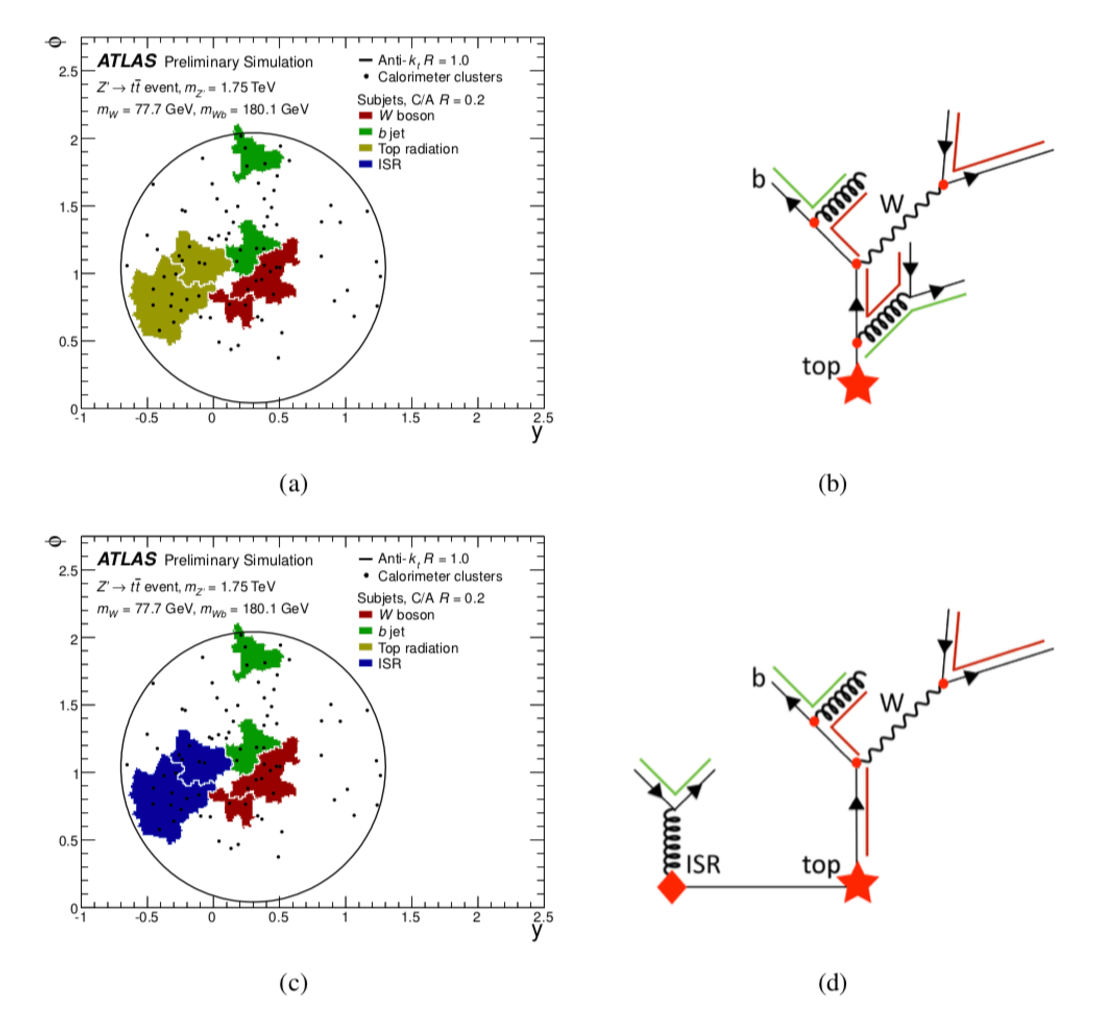
\includegraphics[width=0.79\textwidth]{figures/showerdec_histories.pdf}}
  % 
  \caption{The figure (taken from Ref.~\cite{ATLAS:2014twa})
    illustrates how shower deconstruction works as a top tagger. The
    left-hand panel shows the energy depositions in the
    rapidity-azimuth plane, while the left-hand panel shows the
    corresponding most-likely shower histories. The coloured lines in
    the right panels indicate which partons are colour-connected in
    the respective shower histories.}\label{fig:sd_histories}
\end{figure}


\subsection{HEP top tagger}

The HEP top tagger was first designed to reconstruct mildly boosted
top quarks in a busy event environment, i.e.\ for the reconstruction
of top quarks in the process $pp \to \bar{t} t h$ with semi-leptonic
top quark decays and $\text{H} \to \bar{b}b$~\cite{Plehn:2009rk}. The
hadronically top was expected to be boosted in the $p_t$ range around
250-500~GeV. This first incarnation of the tagger was augmented by
cuts on observables that were manifestly Lorentz-invariant, and thus
boosting between reference frames were no longer necessary. It
proceeds as follows (see Appendix~A of~\cite{Plehn:2010st}): 
\begin{enumerate}
\item one first defines the fat jets with the Cambridge/Aachen
  algorithm with $R=1.5$,
%
\item for a given fat jet jet, one recursively undoes the last step of
  the clustering, i.e. decluster the jet $j$ into subjets $j_1$ and
  $j_2$ with $m_{j_1}>m_{j_2}$, until we observe a mass-drop
  $m_{j_1}<0.8 m_{j}$. When the mass-drop condition is not met, one
  carries on with the declustering procedure with $j_1$.
%
\item For subjets which have passed the mass-drop condition and which
  satisfy $m_j>30$~GeV, one further decomposes the subjet recursively
  into smaller subjets.
%
\item The next step is to apply a filter similarly to what is done by
  the Mass-Drop Tagger. One considers all pairs of hard subjets,
  defining a filtering radius
  $R_{\text{filt}}=\text{min}(0.3,\Delta R_{ij})$. We then add a third
  hard subjet --- considering again all possible combinations --- and apply
  the filter on the three hard subjets keeping (at most) the 5 hardest
  pieces and use that to compute the jet mass.
  % 
  Amongst all possible triplets of the original hard subjets, we keep
  the combination for which the jet mass --- calculated after
  filtering --- gives the mass closest to the top mass and is within a mass window around the true top mass, e.g. in the range $150-200$ GeV.
  % 
\item Out of the 5 filtered pieces, one extracts a subset of 3
  pieces, $j_1$, $j_2$, $j_3$, ordered in $p_t$ and accept it as a
  top candidate if the masses satisfy at least one of the following
  3 criteria:
\begin{align}\label{eq:heptoptagger-cut}
&0.2<\text{arctan}\Big(\frac{m_{13}}{m_{12}}\Big)<1.3
\qquad\text{and}\qquad
R_{\text{min}}<\frac{m_{23}}{m_{123}}<R_{\text{max}}\\
&R_{\text{min}}^2\bigg(1+\frac{m_{13}^2}{m_{123}^2}\bigg)
  < 1-\frac{m_{23}^2}{m_{123}^2}
  < R_{\text{max}}^2\bigg(1+\frac{m_{13}^2}{m_{123}^2}\bigg)
\qquad\text{and}\qquad
\frac{m_{23}}{m_{123}}>0.35\nonumber\\
&R_{\text{min}}^2\bigg(1+\frac{m_{12}^2}{m_{123}^2}\bigg)
  < 1-\frac{m_{23}^2}{m_{123}^2}
  < R_{\text{max}}^2\bigg(1+\frac{m_{12}^2}{m_{123}^2}\bigg)
\qquad\text{and}\qquad
\frac{m_{23}}{m_{123}}>0.35,\nonumber
\end{align}
with $R_{\text{min}}=0.85\, m_W/m_t$ and $R_{\text{max}}=1.15\,
m_W/m_t$.
\item the combined $p_t$ of the 3 subjets constructed in the previous
  step is imposed to be at least 200~GeV.
\end{enumerate}

Physically, the first three steps above try to decompose a massive
object into its hard partons, in a spirit similar to what the
mass-drop condition used in the MassDrop tagger does.
%
The filtering step also plays the same role of further cleaning the
contamination from the Underlying Event as in the MassDrop tagger.
%
Finally, the set of constraints in (\ref{eq:heptoptagger-cut}) is
meant as a cut on the 3-subjets, mimicking a 3-parton system, to match
the kinematics of a top decay and further suppress the QCD
background. The whole procedure can be visualised as shown in Fig.~\ref{fig:heptoptagger}.

%picture taken from:
%https://twiki.cern.ch/twiki/pub/CMSPublic/PhysicsResultsJME13007/HEP_one_slide_description.pdf
\begin{figure}
  \centerline{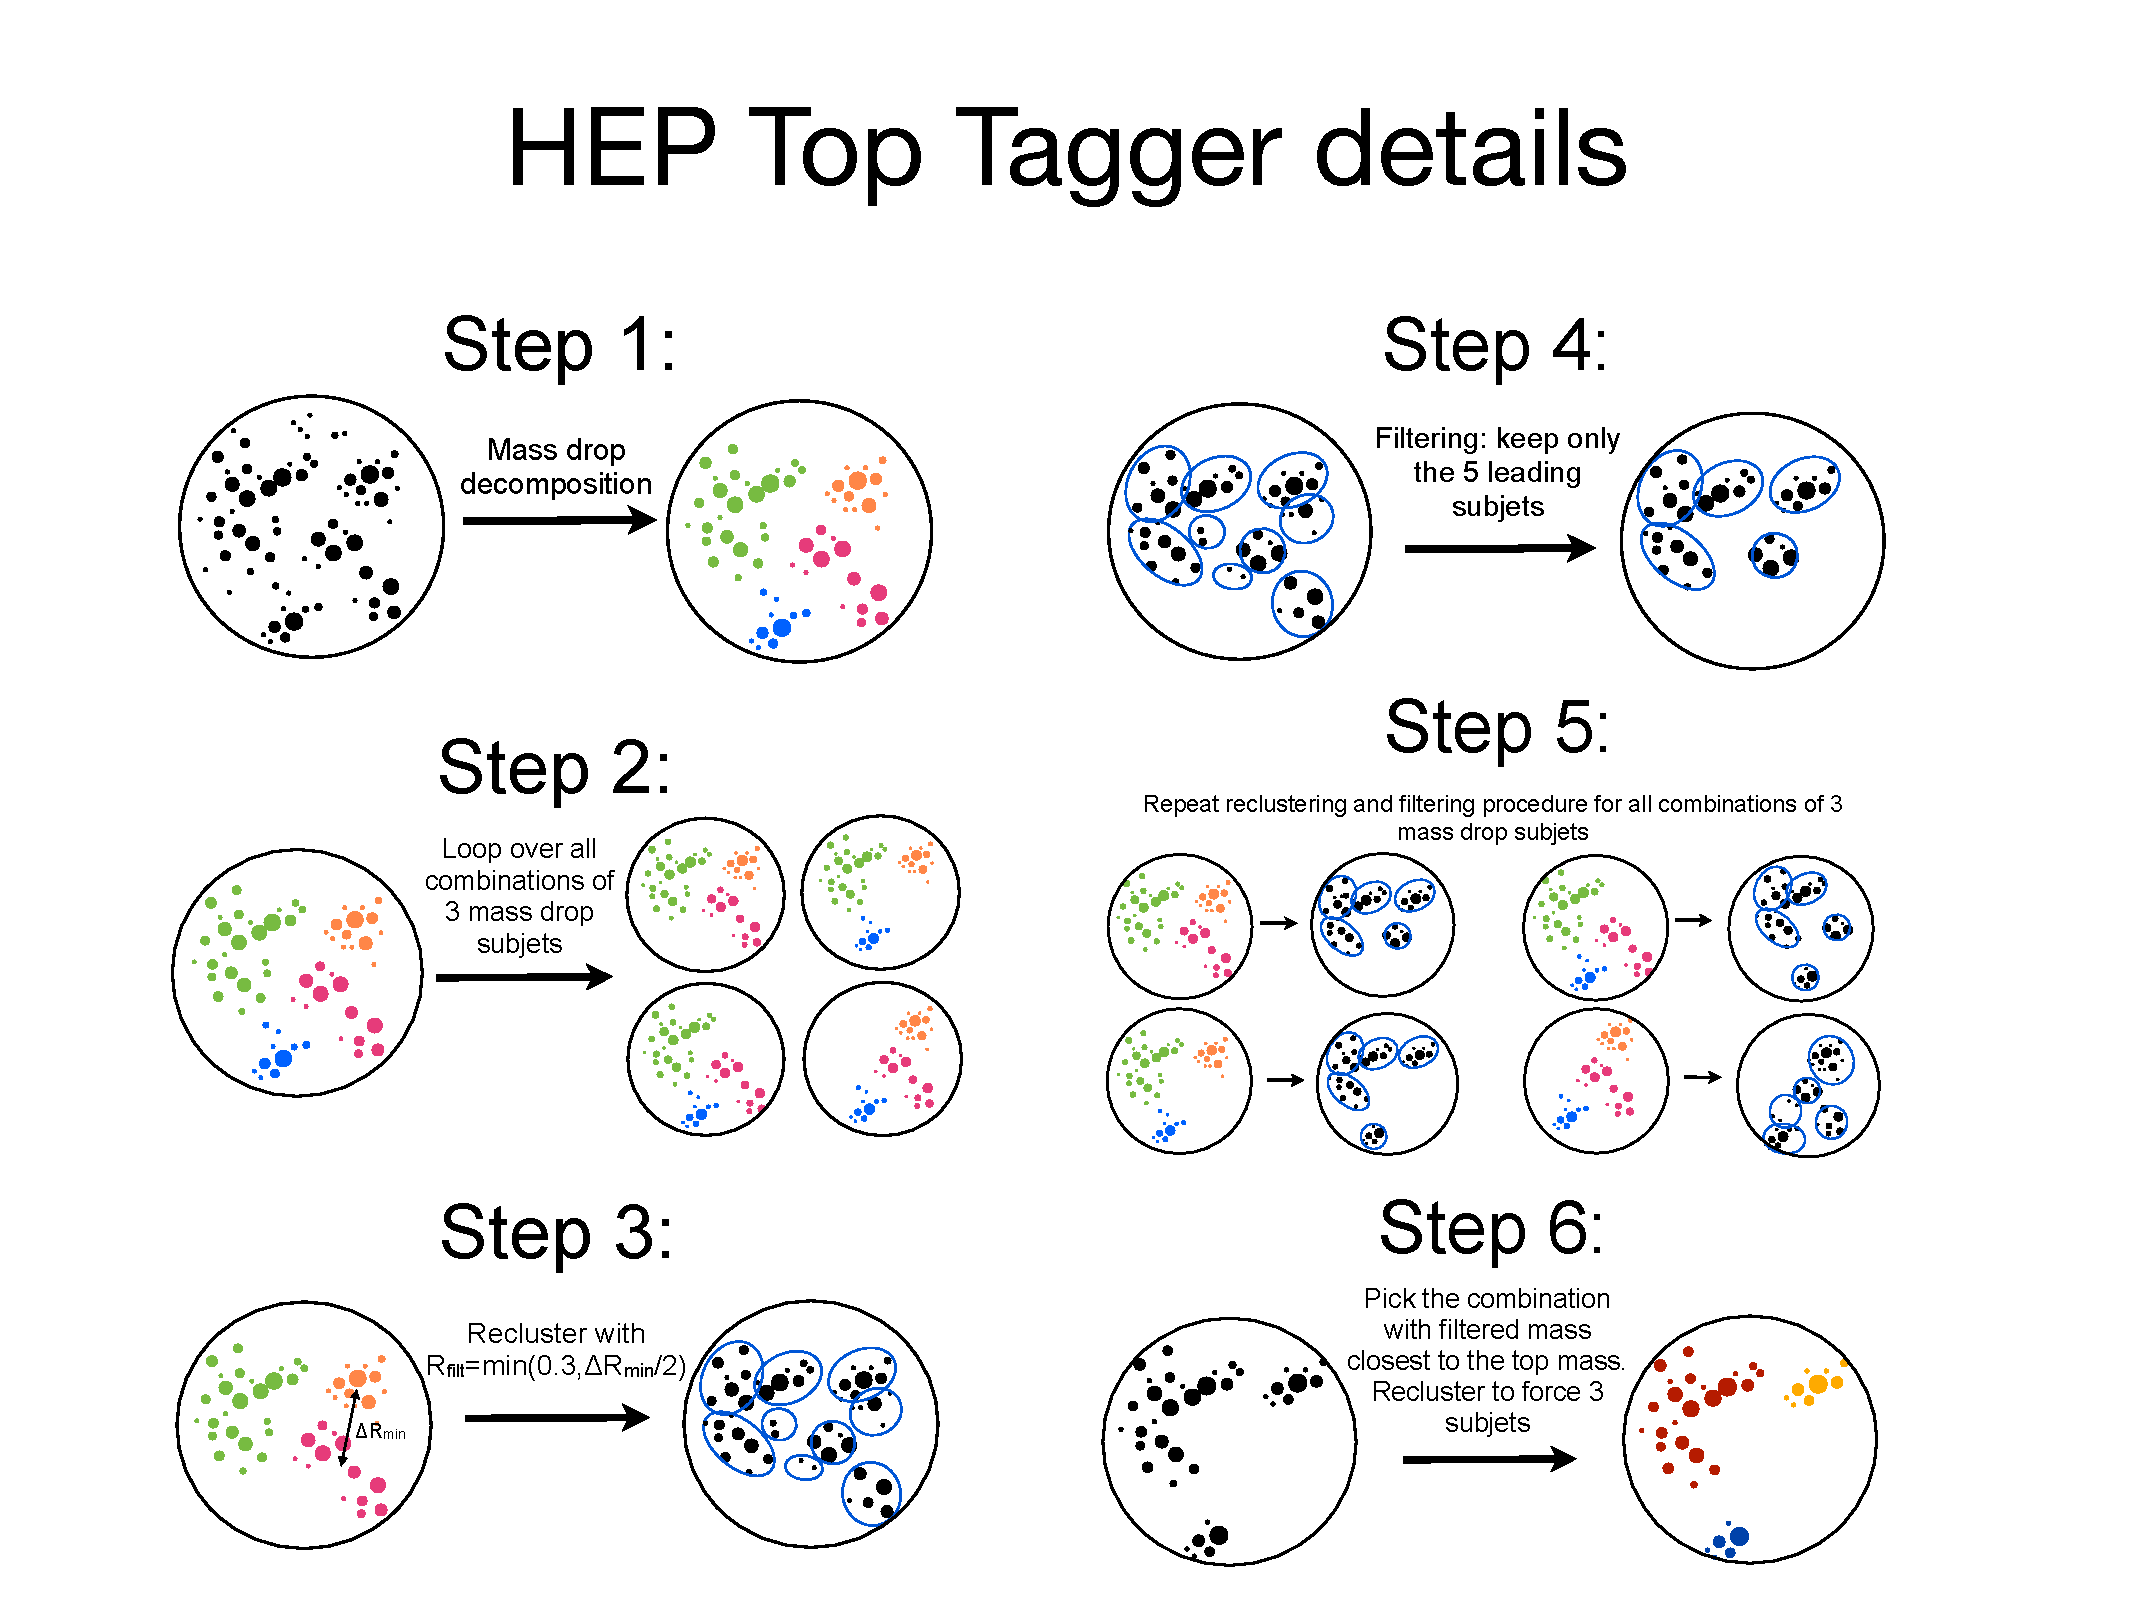
\includegraphics[width=0.65\textwidth]{figures/heptoptagger.pdf}}
  % 
  \caption{Visualisation of the HEP top tagger algorithm.}\label{fig:heptoptagger}
\end{figure}

Version 2 of the HEPTopTagger~\cite{Kasieczka:2015jma} brings several
improvements by using an extended set of variables and cuts. We just
list those modifications without entering into the details.
%
First, it introduces a variable radius by repeatedly reducing the jet
radius, starting from $R=1.5$, until we see a drop in the
reconstructed top mass. This is meant to reduce possible combinatorial
effects where the softest of the W decays is mistaken with a hardish
QCD subjet in the fat top candidate jet.
%
Then, the tagger includes additional shape variables:
\begin{itemize}
\item $N$-subjettiness values for $\beta=1$ computed both on the
  plain, ungroomed, jet and on the filtered jet
\item $Q$-jet information: the reconstructed top mass obtained from
  100 $Q$-jet histories based on the Cambridge/Aachen algorithm with $\alpha=1$,
  as well as the fraction of positive top tags one would obtain with
  version 1 of the HEPTopTagger.
\end{itemize}
% 
In the end, the tagger uses a multivariate (Boosted Decision Tree)
analysis based on the series of kinematic variables --- subjet
transverse momenta and masses --- the optimal jet radius, and the
shape values.

\subsection{The Lund jet plane}

\begin{figure}
  \centerline{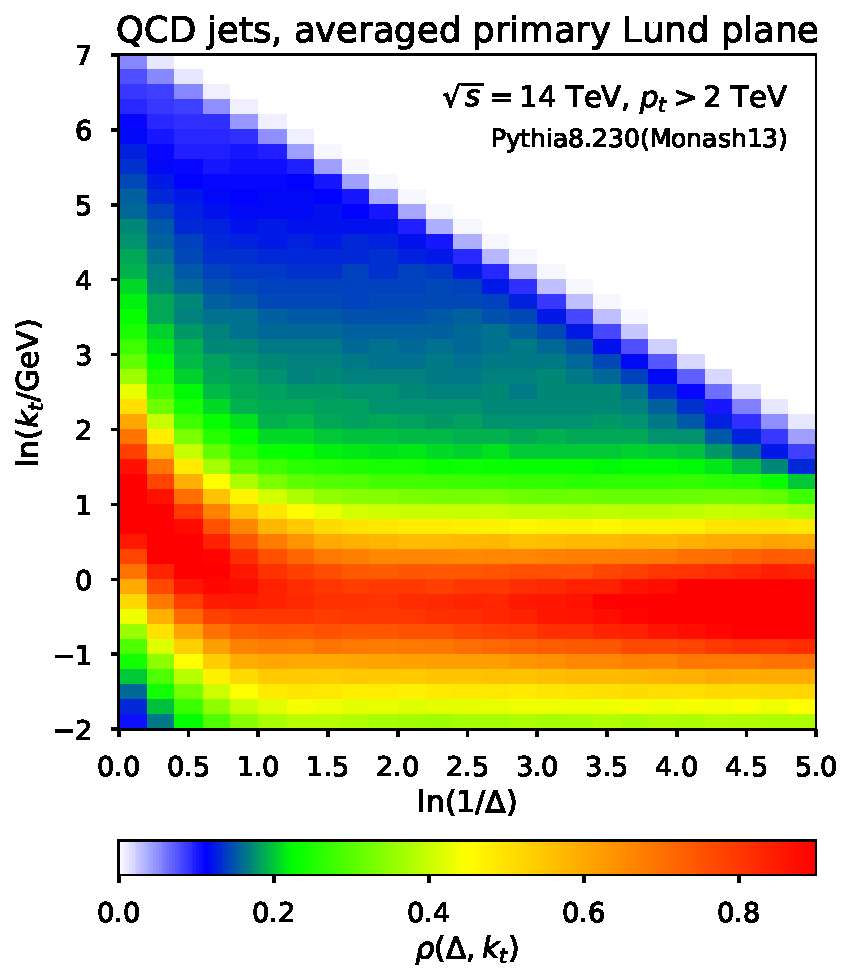
\includegraphics[width=0.5\textwidth,page=1]{figures/plot-Wdiscrim-lund-images.pdf}}
  \caption{The average primary Lund plane density, $\rho$, for jets
    clustered with the C/A algorithm with $R=1$. We selected jets having
    $p_t>2$~TeV and $|y|<2.5$.}\label{fig:lund-primary-plane}
\end{figure}
  

In section~\ref{sec:jet-mass-res}, we have introduced the Lund plane
as a graphical representation convenient for resummation
calculations. It has actually been realised recently that, in the
context of jet substructure, it was possible to promote this idea to a
genuine observable~\cite{Dreyer:2018nbf}.

In practice, one reclusters the constituents of the jet with the
Cambridge/Aachen algorithm and apply the following iterative
procedure, starting with the full jet:
\begin{enumerate}
\item decluster the jet in two subjets $p_i$ and $p_j$, with $p_{ti}>p_{tj}$.
\item with the idea that this corresponds to the emission of $p_j$
  from an emitter $p_i+p_j$, one defines the following variables:
  \begin{align}
    \Delta &\equiv \Delta R_{ij},& k_t&\equiv p_{tj\Delta},&
    m^2&\equiv (p_i+p_j)^2\\
    z&\equiv\frac{p_{tj}}{p_{ti}+p_{tj}}, &\kappa&\equiv z\Delta,&
    \psi&\equiv\tan^{-1}\frac{y_j-y_i}{\phi_j-\phi_i}
  \end{align}
\item Iterate the procedure by going back to step one for the harder
  subjet $p_i$.
\end{enumerate}
This construction produce an ordered list of tuples
\begin{equation}
{\cal {L}}_{\text{primary}} \equiv \big[{\cal {T}}^{(1)},\dots,{\cal
  {T}}^{(n)}\big]
\qquad\text{ with }{\cal {T}}^{(i)}\equiv\big\{\Delta^{(i)},k_k^{(i)},\dots\big\},
\end{equation}
where ${\cal {T}}^{(i)}$ corresponds to the $i$th step of the
declustering procedure.
%
In particular, the set of pairs
$(\log(1/\Delta^{(i)}),\log(k_t^{(i)}))$ corresponds to a
representation of all the primary emissions of a given jet in the
Lund-plane representation of section~\ref{sec:jet-mass-res}
(cf.~Fig.~\ref{fig:lund-plain}). This provides a overview of the
internal structure of the jet.

Fig.~\ref{fig:lund-primary-plane} shows the average Lund plane density
\begin{equation}
\rho(\Delta,k_t) \equiv \frac{1}{N_\text{jet}}\frac{dn_\text{emissions}}{d\log(1/\Delta)d\log(k_t)}
\end{equation}
obtained from Pythia simulations using a dijet event sample. The main
regions labelled in Fig.~\ref{fig:lund-plain} can be clearly
identified in Fig.~\ref{fig:lund-primary-plane}.

As shown in Ref.~\cite{Dreyer:2018nbf}, the Lund jet plane can be used
for measurements and for constraining Monte-Carlo
generators. Furthermore, boosted object taggers can be built from the
Lund plane either via a log-likelihood approach, or using machine
learning techniques.

\section{Code Availability}

An essential component of a successful jet substructure algorithm, is its availability.
%
Therefore, for completeness, we list below where one can find the implementation
of the tools presented above.

\vspace{0.5cm}

\noindent
 \begin{tabular}{lp{9cm}}
  \hline
  {\bf Tool} & {\bf Code} \\
  \hline
  Mass-Drop Tagger          & \ttt{MassDropTagger} class in \fastjet \\
  modified Mass-Drop Tagger & \ttt{ModifiedMassDropTagger} class in the \\
                            & \ttt{RecursiveTools} \fastjet contrib\\
  SoftDrop                  & \ttt{SoftDrop} class in
                              the \ttt{RecursiveTools} \fastjet
                              contrib\\
  Recursive SoftDrop        & \ttt{RecursiveSoftDrop} class in
                              the \ttt{RecursiveTools} \fastjet
                              contrib\\
  Filtering                 & \ttt{Filter} class in \fastjet (use \ttt{SelectorNHardest})\\
  Trimming                  & \ttt{Filter} class in \fastjet\\ & (use \ttt{SelectorPtFractionMin})\\
  Pruning                   & \ttt{Pruner} class in \fastjet\\
  I and Y-Pruning           & Not available per se but can be
                              implemented as a derived class of
                              \ttt{Pruner}\\
  Johns Hopkins top tagger  & \ttt{JHTopTagger} class in \fastjet \\
  CMS top tagger            & as part of CMS-SW (see Ref.~\cite{CodeCMSTopTagger})\\
  Generalised angularities  & no know public standard implementation\\
  $N$-subjettiness          & \ttt{Nsubjettiness} \fastjet contrib\\
  Energy Correlation Functions & \ttt{EnergyCorrelator} \fastjet contrib\\
  HEPTopTagger  & code available from Ref.~\cite{CodeHEPTopTagger} \\
  Shower Deconstruction & code available from Ref.~\cite{CodeShowerDeconstruction} \\
  \hline
\end{tabular}

\vspace{0.5cm}


Let us conclude this chapter with a more general remark.
Grooming techniques
might at first sight be similar to pileup mitigation techniques. They
however target a different goal: while pileup mitigation techniques
aim at correcting for the average effect of pileup, grooming
techniques reduce the overall sensitivity to pileup.
%
In practice, this means that, unless one first applies an event-wide
pileup mitigation technique such as
SoftKiller~\cite{Cacciari:2014gra} or PUPPI~\cite{Bertolini:2014bba},
grooming techniques should in principle be supplemented by pileup
subtraction, like the
area--median~\cite{Cacciari:2007fd,Cacciari:2008gn,AlcarazMaestre:2012vp,Soyez:2012hv}. 
Many tools provide hooks to combine them with pileup subtraction.


%% GS helper for auctex
%%% Local Variables:
%%% mode: latex
%%% TeX-master: "notes"
%%% End:

%  LocalWords:  pronginess performant MassDrop WTA Eq Nsubjettiness
%  LocalWords:  ECFs ij Houches Neyman Eqs HEPTopTagger hardish PUPPI
%  LocalWords:  RecursiveTools contrib JHTopTagger EnergyCorrelator
